% JuliaCon proceedings template
\documentclass{juliacon}
\usepackage{amsmath}
\setcounter{page}{1}

\begin{document}
% **************GENERATED FILE, DO NOT EDIT**************

\title{My JuliaCon proceeding}

\author[1]{1st author}
\author[1, 2]{2nd author}
\author[2]{3rd author}
\affil[1]{University}
\affil[2]{National Lab}

\keywords{Julia, Optimization, Game theory, Compiler}


\maketitle
\begin{abstract}

The aim of this paper is twofold. The first one is to describe a novel research-project designed for building bridges between machine learning and econometric worlds. The second one is to introduce the main characteristics and comparative performance of the first Julia-native all-subset regression algorithm included in \verb GlobalSearchRegression.jl  (v1.0.3). As other available alternatives, this algorithm allows researchers to obtain the best model specification among all possible covariate combinations - in terms of user defined information criteria-, but up to 3165 and 197 times faster than STATA and R alternatives, respectively. 

\end{abstract}

\section{Introduction}
While allowing for better and more accurate analysis (and forecasts), fat-data availability generates a revival of Bellman’s \cite{Bellman1961} -and newer- high-dimensionality concerns:
\begin{enumerate}
    \item Exponential increase in required information and execution time \cite{Yu2003} ;
    \item Overfitting risk \cite{Defernez1999}; 
    \item Less-informative euclidean distances \cite{Aggarwal2001}; and
    \item Unfeasible estimators \cite{Buhlmann2011}. 
\end{enumerate}

Notwithstanding, the advantage of having thousands/millions of features to deal with complex phenomena stimulates an unprecedented number of methodological -and technological- improvements to manage the ‘curse of dimensionality’ \cite{Bolon2016}. \vskip 6pt

In Economics, this process has a dual approach with machine-learning (ML) and econometric (EC) algorithms emerging for different purposes: the former for prediction/forecasts (focusing on $\hat{y}$) and the latter for estimation/causal inference (interested in $\hat{\beta}$). Alternatively, the same distinction can be expressed in Diebold’s terms as non-causal vs causal prediction (see \cite{athey2015}), where ML algorithms are designed to reduce prediction sampling-risks -i.e. learning through cross-validation techniques- and EC methods to identify unbiased multivariate relationships -i.e. avoiding consistency issues through residual and coefficient tests for model selection. \vskip 6pt

In turn, ML feature selection algorithms can be classified into three different families: Filters, Wrappers and Embedded -depending on whether they use some classifier/response variable information or not, or how variable selection is made along with the learning process, see \cite{chandras2014}. Similarly, most EC dimensionality reduction approaches can be classified into three different groups: Exhaustive, General-to-Specific and Specific-to-General -depending on the search pattern; see \cite{gluzmann2015}. \vskip 6pt

Despite significant improvements in recent econometric developments -like PCGIVE/Autometrics or Retina algorithms, which combine some ML and EC characteristics-, available alternatives fails to fully exploit cross-validation and model averaging capabilities -see \cite{Doornik09autometrics}, \cite{perezamaral2003}, \cite{DAVIDSON1981}, \cite{derksen1992}, \cite{marinucci2008}, \cite{herwartz2010}, and \cite{castle2006}. \vskip 6pt

Conversely, newer ML algorithms -like Convolutional Neural Networks or Bootstrap-Based LASSO, which improve complex non-linear adjustment or model selection under regularization schemes- achieved unprecedented forecast accuracy but disregarding model interpretability and/or parameter estimation issues -i.e omitting residual and coefficient tests; see \cite{Bzdok2018}. \vskip 6pt

Following Varian’s \cite{varian2014} advices, about ML and EC complementarities -i.e. merging algorithms from different families to reduce both sampling and model uncertainty-, we are developing a novel multi-layer-multi-algorithm methodology combining two reinforcing paradigms: The LSE “Testimation” approach -to obtain information about residual properties, see \cite{abramovich2006}- and the Bayesian-like “Double-model averaging” -across different covariates and sub-samples, see \cite{hoetening1999}. This methodology includes five complementary layers -handling cross-section, time series and panel data-: 1) Pre-processing: with outlier detection, missing values identification, seasonal adjustment and normalization/standardization functions; 2) Feature extraction: creation of logs, squares, inverses and interactions from selected variables; 3) Feature pre-selection: using filter and embedded ML algorithms like CFS, Variance threshold and LASSO functions; 4) Final feature selection: with a modified all-subset regression approach, including residual tests and model averaging capabilities; 5) Post-estimation fine-tuning: coefficient re-evaluation through cross-validation techniques and model averaging across different k-fold results. \vskip 6pt


The objective of this paper is to introduce the main characteristics and comparative performance of a key layer of our methodology: the modified all-subset 
regression algorithm included in \href{https://github.com/ParallelGSReg/GlobalSearchRegression.jl}{GlobalSearchRegression.jl} (v1.0.3). As other available 
alternatives (like \href{https://cran.r-project.org/web/packages/MuMIn/MuMIn.pdf}{MuMin-pdredge} in R, or \href{https://www.researchgate.net/profile/
Pablo_Gluzmann/publication/264782750_Global_Search_Regression_A_New_Automatic_Model-selection_Technique_for_Cross-section_Time-series_and_Panel-data_Regressions/
links/53eed18a0cf23733e812c10d/Global-Search-Regression-A-New-Automatic-Model-selection-Technique-for-Cross-section-Time-series-and-Panel-data-Regressions.pdf?
origin=publication_detail}{GSREG} Stata alternatives), this Julia algorithm allows researchers to obtain the best model specification among all possible 
covariate/feature combinations - in terms of user defined information criteria-, but up to 3165 times faster than Stata and 197 times faster than R. \vskip 6pt

\section{Package's main features}
\label{sec:packagefeatures}

Written in Julia, GlobalSearchRegression is a parallel (and improved) version of the Stata-GSREG all-subset regression command (get the original code \href{https://ideas.repec.org/c/boc/bocode/s457737.html}{here}). The package structure is quite simple, as shown in figure 1:


%%%%%%%%%%%%%%%%%% Figure 1
\begin{figure}[h]
\centerline{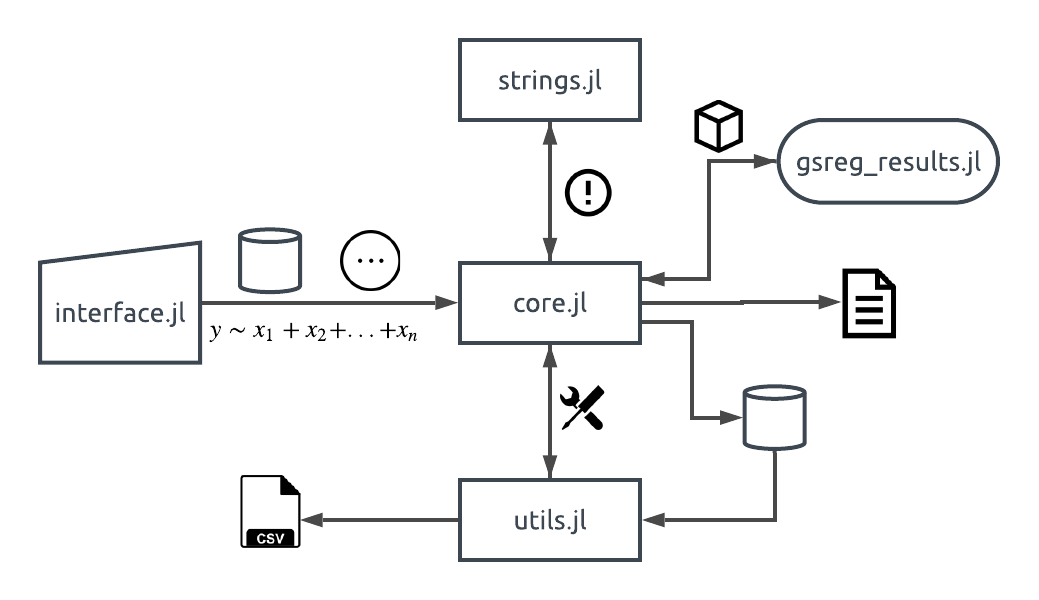
\includegraphics[width=10cm]{flowchart.png}}
\caption{ GlobalSearchRegression.jl Structure Flowchart}
	\label{fig:sample_figure}
\end{figure}
%%%%%%%%%%%%%%%%%%%%%%%%%%%

Through the gsreg function of the \verb interface.jl  internal package, users set the appropriate database to be used, the general unrestricted model -GUM, which defines the search space- and additional options for model selection. With this information and complementary supporting functions and definitions provided by \verb strings.jl  -i.e. error messages-, \verb utils.jl  -i.e. equation formatting, combinatorial analysis, database manipulation, sorting results, etc.- and \verb gsreg_results.jl  -i.e. the structure to save estimation results-, the \verb core.jl  package perform the all-subset-regression algorithm explained in the pseudocode below, to obtain the following outputs: 1) a matrix -optionally exported to a csv file through \verb utils.jl-  including egression coefficients, selection criteria, observations and (optionally) t-test, residual tests, averaging-weights and out-of-sample metrics for every lternative model; 2) a text file -also displayed on screen- which contains the best model specification and (optionally) model averaging results in terms of he user-selected information criteria -see multiple examples in \verb runtest.jl-. \vskip 6pt
\break

%%%%%%%%%%%%%%%%%%%%%%%%%%%%%%%%%%%%%%%%%%%%%
% INSERT PSEUDOCODE HERE IN TABLES OR FIGURES
%%%%%%%%%%%%%%%%%%%%%%%%%%%%%%%%%%%%%%%%%%%%%


\section{Comparative performance against \textit{R} and \textit{STATA}}
\label{sec:comparativeperf}

In table 1, we present a performance comparison of our GLobalSearchRegression Julia-package against its main alternatives: MuMin-pdredge and GSREG (written in  and Stata\footnote{The parallel version of Stata-GSREG is still under development. A preliminary version is available upon request from authors}, espectively).
Execution times were obtained from a HED architecture using a Threadripper 1950x build, with 16 cores (32 threads) overclocked to 3.8GHz and 64 GiB of DDR4-RAM at 3200Mhz. Comparative scripts were implemented on Julia 1.0.3, R 3.6.0 and Stata 15 IC, running on Ubuntu 18.04.2 LTS -Linux kernel 4.15-\footnote{All these test are available \href{https://github.com/ParallelGSReg/GlobalSearchRegression.jl/tree/master/juliacon2019proceedings/reproducibility}{here}} \vskip 6pt

For experimental -random variable- databases with a few covariates -up to 15 explanatory variables-, our Julia algorithm only provides significant time improvement in standard personal computers -e.g. 4 cores-, being up to twice faster than R and 4 times faster than Stata. For HED computers or HPC nodes, there is almost no difference among the best result obtained for each alternative. \vskip 6pt


However, for databases with 20 or more covariates, our Julia all-subset-regression code is always faster, irrespective of the number of observations or threads -up to 3165 times faster than STATA and 197 times faster than R-. Execution time differences exponentially increase with the number of covariates and slightly decrease with available observations. Moreover, Stata and R alternatives become unfeasible for databases with 25 or more covariates. For a confirmatory nalysis,in figure 2 we present execution-time kernel densities for the 20 covariates - 100 observations - 32 threads case, obtained from 300 independent non-cached) runs. Kernel results show that execution time differences are not an artifact obtained from noisy runs. Our Julia algorithm is consistently faster han R and Stata alternatives. \vskip 6pt

A detailed speed-up analysis is also available for the 25-covariate case. In figure 3, it's shown that our Julia all-subset-regression algorithm scales almost linearly for large databases -while the number of threads is not higher than the number of physical cores-. With small databases, Amdhal's law \cite{Amdahl1967}inputs change. Parallel tasks become lighter and speed-up efficiency degrades consistently with additional threads, because the marginal overhead cost of a larger environment creation is not overcompensated by parallelism gains obtained from additional threads. Notwithstanding, using only physical cores speed-up efficiency is always above 45 \%  -with an average of 84\% for 2, 4, 8 and 16 threads-. 

%%%%%%%%%%%%%%%%%%%%%%%%%%%%%%%%%%%%%%%%%%%%%%%%%%%%%%
% INSERT PSEUDOCODE HERE  FIGURES 2 and 3
%%%%%%%%%%%%%%%%%%%%%%%%%%%%%%%%%%%%%%%%%%%%%%%%%%%%%%


\section{Why GlobalSearchRegression.jl is faster than existing alternatives?}
\label{sec:whygsreg}
\subsection{JULIA platform}
\label{subsub:juliaplat}

Despite some \verb GlobalSearchRegression.jl  specific features to be examined below, our all-subset-regression algorithm benefits from the well-known Julia language efficiency for High Performance Computing tasks.


%%%%%%%%%%%%%%%%%%%%%%%%%%%%%%%%%%%%%%%%%%%%%%%%%%%%%%
% INSERT PSEUDOCODE HERE TABLE 2
%%%%%%%%%%%%%%%%%%%%%%%%%%%%%%%%%%%%%%%%%%%%%%%%%%%%%%

Julia JIT-compilation allows packages to run faster than those executed using interpreted or byte-compiled languages (like R or Stata-Mata). Indeed, basic functions running on Julia can be up to 251 and 368 times faster than those running in R and Stata, respectively -with an average speed-up of 75 and 90, see Table 2-.

\subsection{Parallel strategy and memory setup}
\label{subsub:parallelst}

It is well know that multicore architectures can be used to speed-up execution times through two main paradigms: data and task-parallelism \cite{zaki2001}. The preferred strategy critically depends on:
\begin{enumerate}
    \item Database structure;
    \item Algorithm serial portion; and
    \item Interthread communication costs.
\end{enumerate} 

The first discussion is about tall vs fat data. While tall databases are more suitable for data-parallelism \cite{babu2013}, fat-structures improve relative performance of task-parallelism (because tasks increase exponentially with covariates/columns in feature selection problems, see \cite{foster1994}). \vskip 6pt

Additionally, the choice between alternative paradigms takes into account the Amdahl's Law for the specific algorithm to be used. Task-parallelism is usually better for econometric and machine learning algorithms requiring some specific serial optimization paths (i.e. arima-arfima models), while data-parallelism performs better under linear-algebra solutions (i.e. OLS-family estimators, see \cite{guo2012}). \vskip 6pt

Finally, we have the problem of intercomunication costs. Data-parallelism -generally- involves intense needs of inter-thread-communication. While task-parallelism communication costs depends on Load-Balancing choices (i.e. Dynamic vs Static), they are usually lower than data-parallelism ones \footnote{At least when Static Load Balancing is implemented, because it allows for Coarse-grained granularity \cite{gordon2006}} \cite{MOREANO2017}. \vskip 6pt

For feature selection problems, pros and cons of alternative strategies often determine that available cores should be used for task parallelism. Databases are fat, data-mining algorithms can include large serial portions, and intercomunication costs can be huge for large-multicore architectures. These reasons explain why all available all-subset-regression packages use taks-parallism to speed-up execution times. \vskip 6pt

As for the memory setup, there are also alternative methodologies. First, it's necessary to choose among Static vs. Dynamic memory allocations \cite{prajapati2015}. To improve speed-up, Static "once-and-for-all" allocations are often preferred (even at a cost of higher average memory utilization). Second, shared-memory strategies must be determined. Depending on both object-size and CPU architecture -cache size and its distribution among cores-, it could be optimal to use large shared arrays or -alternatively- smaller core-specific objects. Splitting output matrices to work with smaller non-shared arrays could be useful for cache optimization purposes, but it could also entail additional communication costs and higher memory requirements \cite{ahmed2015}. In practice, feature selection algorithms usually prefer shared-arrays for high performance computing. \vskip 6pt

\verb GlobalSearchRegression.jl  (execution-time) advantages have been obtained combining:
\begin{itemize}
    \item[a)]  Task-parallelism
    \item[b)]  Static Load-Balancing
    \item[c)]  Coarse-grained granularity   
    \item[d)]  Static memory allocation
    \item[e)]  Efficient shared-array implementation
\end{itemize}

While some of these characteristics are shared with R and Stata alternatives (\verb MuMin-pdredge  and \verb GSREG,  respectively), our Static Load-Balancing algorithm outperform the round-robin R scheduling (implemented by the clusterapply function included in the \verb parallel  R-package see \cite{deb2013}) and the Shared-Array strategy significantly improves I/O performance against Stata. By construction, pure Static Load-Balancing in GlobalSearchRegression.jl avoids Round-Robin communication costs and execution gaps. This advantage overcompensate minimal\footnote{Minimal because our static scheduler guarantees that average task-complexity will not be too different among workers} load-asymmetries, associated with any static scheduling. In turn, using efficient shared-arrays to store all-subset-regression results allows us to outperform the \verb Stata-GSREG  methodology which heavily relies on slower I/O disk operations (because multiple instances must be launched to enable task-parallelism and, therefore, shared-arrays become unfeasible). \vskip 6pt

\subsection{OLS estimation}
\label{subsub:ols}

Efficient Ordinary Least Squares (OLS) algorithms rely on Linear Algebra operations (matrix decomposition, matrix inversion, etc.).\footnote{Optimization alternatives (i.e. Gradient descent), while quite inefficient for linear models, can also be used for non-linear estimations \cite{abdi2007}} The traditional $(X'X)^{-1}$ operation could be time-expensive with unstable solutions under certain conditions \cite{jameson1981}. A preferred method is the QR-decomposition developed by Francis \cite{francis1961} and Kublanovskaya \cite{kublanovskaya1962s}. The QR factorization allows us to decompose any full rank $N \times p$ matrix $\bar{X}$ as:


% **************GENERATED FILE, DO NOT EDIT**************

\bibliographystyle{juliacon}
\bibliography{ref.bib}
\end{document}

% Inspired by the International Journal of Computer Applications template
